\documentclass{article}  % Define la clase del documento.

% Paquetes de idioma y codificación
\usepackage[utf8]{inputenc}
\usepackage[T1]{fontenc}
\usepackage[spanish]{babel}  % Ajusta el idioma del documento a español.

% Paquete de geometría para configurar márgenes y tamaño de papel
\usepackage[letterpaper, margin=3cm]{geometry}

% Paquetes de tipografía
\usepackage{mathptmx}    % Usa Times New Roman como fuente.
\usepackage{microtype}   % Mejora la justificación del texto.

% Paquetes para manejo de colores y gráficos
\usepackage{xcolor}      % Define y utiliza colores.
\usepackage{graphicx}    % Permite la inserción de imágenes.
\usepackage{tikz}        % Creación de gráficos vectoriales.

% Configuración de enlaces y referencias cruzadas
\usepackage{hyperref}
\hypersetup{
    colorlinks   = true,
    linkcolor    = darkblue,
    citecolor    = black,
    filecolor    = blue,
    urlcolor     = blue
}

% Paquetes para la mejora visual de tablas y figuras
\usepackage{booktabs}    % Para tablas de alta calidad.
\usepackage{float}       % Controla la posición de figuras y tablas.

% Paquete para la personalización de códigos fuente
\usepackage{listings}
\lstset{
    literate=
    {á}{{\'a}}1 {é}{{\'e}}1 {í}{{\'i}}1 {ó}{{\'o}}1 {ú}{{\'u}}1
    {Á}{{\'A}}1 {É}{{\'E}}1 {Í}{{\'I}}1 {Ó}{{\'O}}1 {Ú}{{\'U}}1
    {ñ}{{\~n}}1 {Ñ}{{\~N}}1 {ü}{{\"u}}1 {Ü}{{\"U}}1,
    backgroundcolor=\color{backcolour},
    commentstyle=\color{codegreen},
    keywordstyle=\color{codepurple},
    numberstyle=\tiny\color{codegray},
    stringstyle=\color{red},
    basicstyle=\ttfamily\small,
    breakatwhitespace=false,
    breaklines=true,
    captionpos=b,
    keepspaces=true,
    numbers=left,
    numbersep=5pt,
    showspaces=false,
    showstringspaces=false,
    showtabs=false,
    tabsize=2,
    language=TeX,
    morecomment=[l]\#,
    frame=single,
    rulecolor=\color{black}
}

% Definición de colores al estilo Visual Studio Code
\definecolor{darkblue}{rgb}{0.0, 0.0, 0.55}  % Enlaces
\definecolor{codegreen}{rgb}{0.25, 0.49, 0.48}  % Comentarios
\definecolor{codegray}{rgb}{0.5, 0.5, 0.5}  % Números y anotaciones
\definecolor{codepurple}{rgb}{0.58, 0, 0.82}  % Palabras clave
\definecolor{backcolour}{rgb}{0.95, 0.95, 0.92}  % Fondo de código

% Configuraciones de párrafo y matemáticas
\usepackage{amsmath}
\usepackage{parskip}    % Espaciado entre párrafos.
\usepackage{ragged2e}   % Justificación mejorada.

% Configuración de secciones y encabezados
\usepackage{titlesec}
\titleclass{\part}{top} % Make part like a class
\titleformat{\part}[display]
  {\normalfont\huge\bfseries\centering}{\thepart}{20pt}{\Huge}
\titlespacing*{\part}{172.5pt}{-60pt}{10pt}
\titleformat{\part}
  {\normalfont\huge\bfseries}{}{0pt}{}

% Asegúrate de usar esto para mantener el estilo en las páginas de las partes
\titleformat{\part}[display]
  {\normalfont\huge\bfseries}{}{0pt}{}
  [\thispagestyle{fancy}] % Aplica el estilo fancy a las páginas de las partes

% Configuración de encabezados y pies de página personalizados
\usepackage{fancyhdr}
\pagestyle{fancy}
\fancyhf{}
\fancyhead[L]{\raisebox{0.20cm}{\textbf{Apuntes Prueba 1 Hidrologia}}}
\fancyhead[R]{\raisebox{0.1cm}{
\includegraphics[width=0.25\linewidth]{LOGO_UNIVERSIDAD.jpg}}}
\fancyhead[C]{\rule{\textwidth}{0.6pt}}
\fancyfoot[C]{\rule{\textwidth}{0.6pt}}
\fancyfoot[R]{\raisebox{-1.5\baselineskip}{\thepage}}
\renewcommand{\headrulewidth}{0pt}
\renewcommand{\footrulewidth}{0pt}

% Configuración avanzada de geometría
\geometry{
  top=3.5cm, % Aumenta el espacio en la parte superior para subir el encabezado
  bottom=2.5cm,
  headheight=2.5cm % Aumenta la altura del encabezado si es necesario
}

% Configuracion de bibliografia
\usepackage{natbib}
\bibliographystyle{unsrtnat}  % Puedes cambiarlo por `unsrtnat`, `abbrvnat`, etc.

\begin{document}
%----------------------------------------------------------------------------------------
% PORTADA
%----------------------------------------------------------------------------------------
\begin{titlepage}%Inicio de la carátula, solo modificar los datos necesarios
\newcommand{\HRule}{\rule{\linewidth}{0.5mm}} 
\center 
%----------------------------------------------------------------------------------------
%	ENCABEZADO
%----------------------------------------------------------------------------------------

\includegraphics[width=10cm]{LOGO_UNIVERSIDAD.jpg}\\ % Si esta plantilla se copio correctamente, va a llevar la imagen del logo de la facultad.OBS: Es necesario incluir el paquete: graphicx
\vspace{3cm}
%----------------------------------------------------------------------------------------
%	SECCION DEL TITULO
%----------------------------------------------------------------------------------------
\HRule \\[0.4cm]
{ \huge \bfseries Apuntes Prueba 1}\\[0.4cm] % Titulo del documento
{ \huge \bfseries Hidrologia}\\[0.4cm] % Titulo del documento
\HRule \\[1.5cm]
 \vspace{5cm}
%----------------------------------------------------------------------------------------
%	SECCION DEL AUTOR
%----------------------------------------------------------------------------------------
\begin{flushright}
    { 
    \textbf{Autores:} \\
    Lukas Wolff Casanova\\
}
\end{flushright}
\vspace{1cm}
%----------------------------------------------------------------------------------------
%	SECCION DE LA FECHA
%----------------------------------------------------------------------------------------
{\large \textbf{\today}}\\[2cm] % El comando \today coloca la fecha del dia, y esto se actualiza con cada compilacion, en caso de querer tener una fecha estatica, reemplazar el \today por la fecha deseada
\end{titlepage}
%----------------------------------------------------------------------------------------
%  INDICE
%----------------------------------------------------------------------------------------
\newpage
\thispagestyle{empty} % Deshabilita el número de página en la página del índice
\tableofcontents
\thispagestyle{plain} % Deshabilita el encabezado en la página del índice
\thispagestyle{empty} % Deshabilita el número de página en la página del índice
\newpage

\newpage
\thispagestyle{empty}
\listoffigures 
\thispagestyle{plain} % Deshabilita el encabezado en la página del índice %
\thispagestyle{empty}
\newpage
%----------------------------------------------------------------------------------------
%ACÁ EMPIEZA EL INFORME
\setcounter{page}{1}
%----------------------------------------------------------------------------------------
\part{Capitulo 1}

\section{El Agua}

El agua es el recurso mas importante y con mayor abundancia del planeta.
Aun asi, su consumo se multiplico por 6 durante el siglo XX.

Algunos datos:

\begin{itemize}
    \item 97.5\% del agua es salada
    \item 2.5\% es dulce
    \item 70\% de esta agua dulce esta en forma de hielo
    \item 30\% esta en acuiferos
    \item 0.3\% esta en rios y lagos
    \item 70\% de la superficie del planeta es agua
    \item 69\% del agua es utilizada en el sector agropecuario
    \item 19\% en la industria
    \item 12\% en el sector municipal
\end{itemize}

\subsection{Uso del Agua en Chile}

\begin{itemize}
    \item 73\% del agua es utilizada en la agricultura
    \item 12\% en la industria
    \item 9\% en la mineria
    \item 6\% en el sector sanitario
\end{itemize}

\section{Hidrologia}

La Hidrología es la ciencia que trata de las aguas de la
Tierra, su existencia, circulación y distribución, sus
propiedades físicas, químicas y sus reacciones con el medio
ambiente, incluyendo su relación con los organismos vivos

\subsection{Objetivos}

\begin{itemize}
    \item Determinacion de la disponibilidad de recursos hidricos
    \item Efectuar estudios de crecidas
\end{itemize}

\section{Ciclo Hidrologico}

\begin{figure}[H]
    \centering
    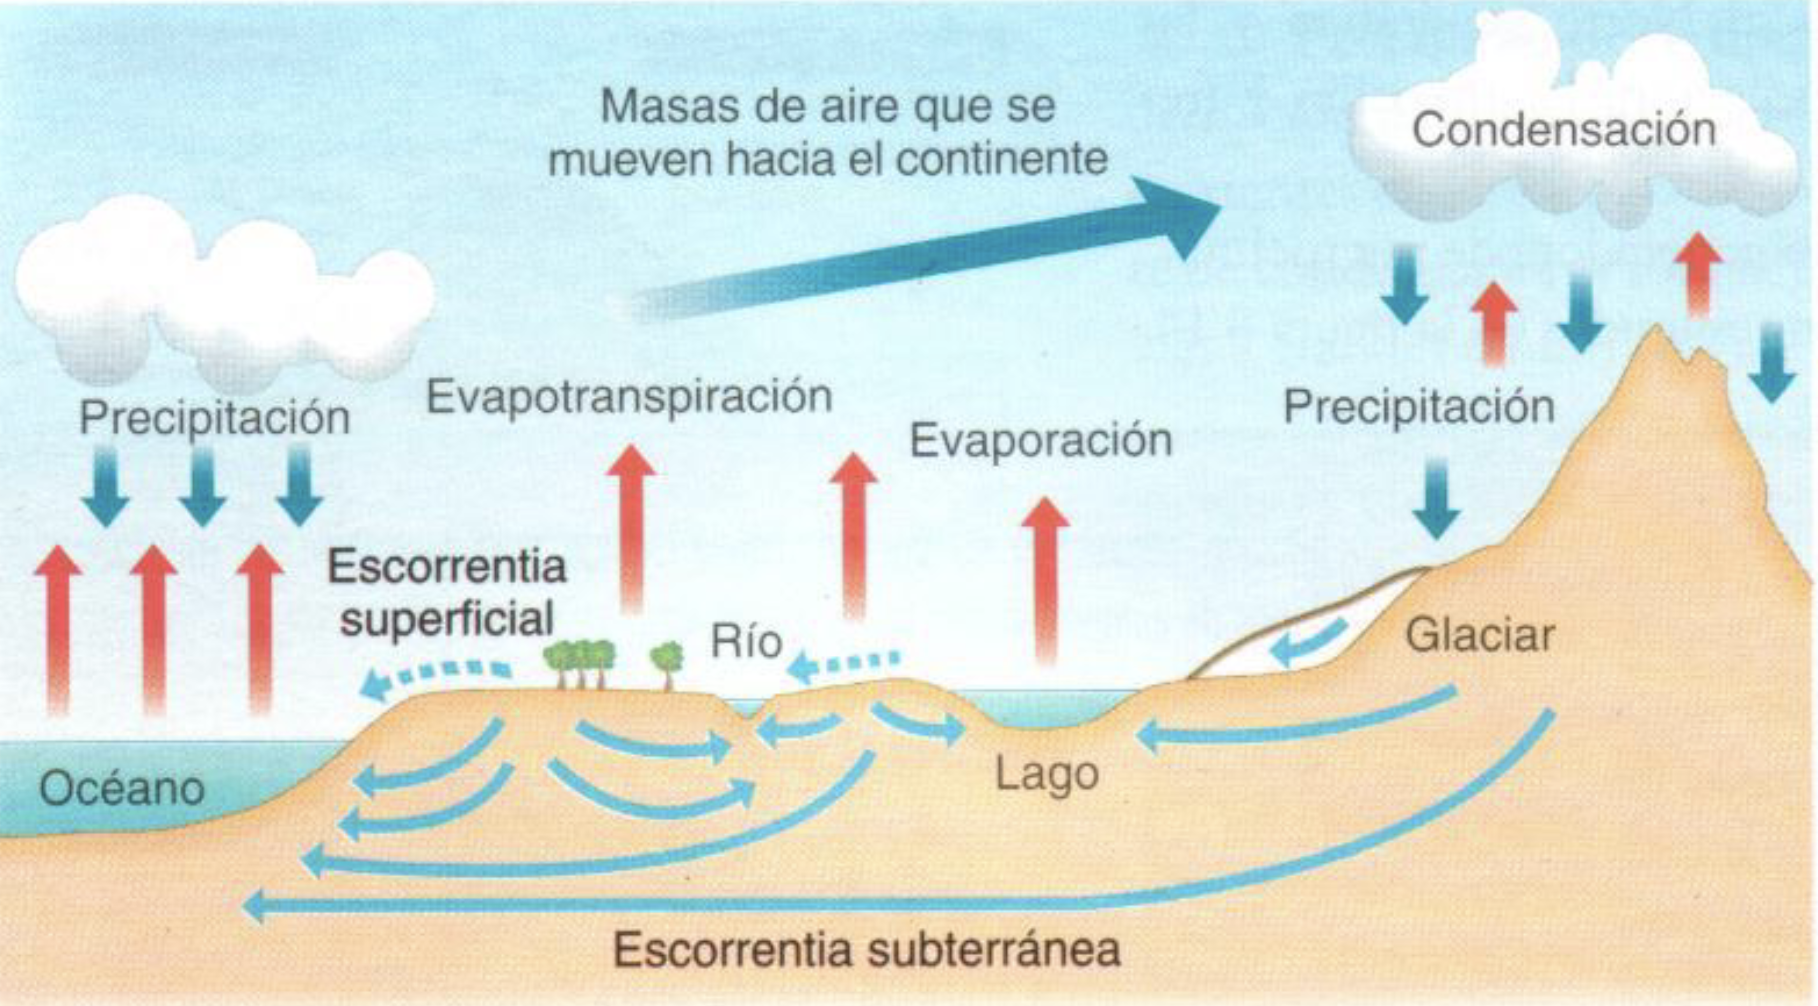
\includegraphics[width=0.85\textwidth]{imagenes/ciclo_hidrologico.png}
    \label{fig:ciclo_hidrologico}
\end{figure}

Se determina la precipitacion como \textbf{Pp}, evaporacion como \textbf{Ev} y la escorrentia como \textbf{Pp-Ev}.

\part{Capítulo 2}
\section{Ciclo hidrológico}
\begin{itemize}
    \item Idealización del movimiento, distribución y circulación del agua en la Tierra, entre la atmásofera-litosfera-hidrósfera y nuevamente a la atmósfera.
    \item Es un sistema complejo
    \item \textbf{Abstracción}: se considera sólo aquellos elementos del ciclo que son posibles de cuantificar
    \item Precipitación, radicación solar y gravedad $\rightarrow$ \textbf{Procesos del ciclo de escorrentía} $\rightarrow$ Evaporación y evotranspiración, escorrentía superficial y escorrentía subterránea.
\end{itemize}

\section{Sistema hidrológico}
Se define como una estructura o volumen en el espacio, rodeada por una frontera, que acepta agua (lluvia), opera en ellas internamente y las produce ccomo salida (caudal).

\begin{itemize}
    \item \textbf{Estructura}: Son los "caminos" del flujo a través de los cuales el agua puede pasar como materia prima desde el punto que entre hasta el punto en que sale.
    \item \textbf{Frontera}: Es una superficie continua definida en 3D, en que encierra el volumen o estructura
\end{itemize}

\subsection{Cuenca u hoya hidrográfica}
Es una superficie de terreno que drena hacia una corriente en un lugar determinado. La \textbf{divisoria de cuencas} es la línea que separa la superficie de la tierra cuyo drenaje fluye hacia un río dado de las superficies de la tierra cuyos desagües corren hacia otros ríos.

La frontera del sistema se dibuja alrededor de la cuenca proyectando la divisoria de aguas verticalmente hacia, y abajo hacia planos horizontales.

\subsubsection{Características geomorfológicas de una cuenca}
\begin{itemize}
    \item Área aportante o superficie (A)
    \begin{itemize}
        \item Corresponde a la proyección en un plano horizontal de la cuenca
    \end{itemize}
    \item Perímetro
    \begin{itemize}
        \item Corresponde a la longitud perimetral de la línea divisoria proyectada
    \end{itemize}
    \item Longitud del cauce principal ($L_c$)
    \begin{itemize}
        \item Corresponde a la medición directa de  la longitud del cuace principal de la cuenca a lo largo de su trayectoria
    \end{itemize}
    \item Longitud del cauce desde centro de gravedad del la cuenca ($L_G$)
    \begin{itemize}
        \item Es la longitud desde el centro de gravedad hasta el punto de salida (Punto control). Una vez indentificado el centroide geométrico se procede a medir la lonfitud del recorrido de una partícula imaginaria de agua, desde este punto hasta la salida de la cuenca.
        \item Centroide geométrico(Cg)
        \begin{itemize}
            \item Centro de gravedad del área de drenaje
        \end{itemize}
    \end{itemize}
    \item Altitud media ($Hm$)
    \begin{itemize}
        \item Corresponde al promedio simple entre la mayor y menor altura del cauce principal.
    \end{itemize}
    \item Pendidente media de la cuenca (S)
    \begin{itemize}
        \item Este parámetro caracteriza en gran parte la  velocidad con que se da la escorrentía superficial afectando el tiempo que lleva el agua de la lluvia para concentrarse en los lechos fluviales que constituyen la red de drenaje de las cuencas.
        \begin{equation}
            S = \frac{\Delta H}{A} \cdot (\frac{l_o}{2} + \sum L_i + \frac{l_n}{2})
        \end{equation}
        \begin{itemize}
            \item $\Delta H$: Desnivel entre curvas de nivel adyacentes, en (m)
            \item $A$: Área de la cuencia en ($m^2$)
            \item $l_o$: Longitud del cauce principal
            \item $L_i$: Longitud de la curva de nivel i
            \item $n$: Número toral de curvas de nivel consideradas
        \end{itemize}
    \end{itemize}
    \item Pendiente media del cauce principal (i)
    \begin{itemize}
        \item Diferencia total entre la cotras del lecho del río, divido por la longitud entre esos dos puntos.
        \begin{equation}
            Y = \frac{Z_{max}-Z_{min}}{L}
        \end{equation}
    \end{itemize}
    \item Curva hipsométrica
    \begin{itemize}
        \item Curva que representa las superficies dominadas por encima de cada curva de nivel y, por lo tanto, caracteriza al relieve de la cuenca.
    \end{itemize}
\end{itemize}

\section{Balance hidrológico}   
Se basa en la aplicación detallada de la ecuación general de balance de masa, sobre una porción de superficie.

\begin{equation}
    \frac{dS}{dt} = X_{Entrada} - Y_{Salida}
\end{equation}

Ecuación general:
\begin{equation}
    P + Q_{SA} + Q_{ZA} - (E + ET + Int + Q_{SE} + Q_{ZE}) = \Delta S_L + \Delta S_S + \Delta S_Z + \Delta S_N
\end{equation}

\textbf{Todo esto está en la ayudantía 1}

\subsection{Fórmula de Turc}
\begin{equation}
    D = \frac{P}{\sqrt{0.9+(\frac{P}{L})^2}}
\end{equation}
Donde:
\begin{itemize}
    \item D: Profundidad de la lluvia en mm, es equivalente a ET
    \item P: Precipitación en mm
    \item $L= 300 +25T +0.05T^3$
    \item T en °C
\end{itemize}

\section{Isolineas de temperatura media anual}

\section{Criterios elección modelos}
\begin{itemize}
    \item \textbf{Respuesta a modos globales de variablidad climática}: Se buscó aquellos modelos que representaban adecuadamente fenómenos interanuales como la influencia de El niño Oscilación del Sur y el Modo Anular del Hemisferio Sur, debido a su influencia en la variablilidad de precipitación en Chile.
    \item \textbf{Sensibilidad climática}: Condición del modelo que hace alusión a la respuesta global del sistema climático a una cierta forzante externa
    \item \textbf{Cambios regionales}: Los cambios proyectados de temperatura y precipitación fueron evaluados para cada modelo. Se seleccionó un conjunto de modelos con impactos diversos
\end{itemize}

\subsection{Criterios escalamiento}
\begin{itemize}
    \item Los enfoques de escalamiento estadístico se basan en el supuesto de establecer relaciones estadísticas entre la información de los GCM y los datos observados, tanto entre ellos como entre los distintos periodos de tiempo a analizar
    \item Escalamiento lineal
    \begin{itemize}
        \item Corrige el modelo por la relación entre las medias de los modelos y de los registros observados
    \end{itemize}
    \item Quantile Delta Mapping (QDM)
    \item 
\end{itemize}






\part{Capitulo 3}
\vspace{-0.3cm}

\begin{center}
    \begin{large}
        Elementos de Meteorología
    \end{large}
\end{center}

La meteorología es la ciencia que estudia los fenómenos ocurridos en la atmósfera (vientos, presipitaciones, etc). Puede estar enfocada en el clima a largo o corto plazo.

\begin{itemize}
    \item Clima (largo plazo): Promedio de las condiciones que se mantienen en un periodo años y esta definido por medias de tendencia central (media, mediana, etc) o variabilidad (rango, desviación estándar, etc).
    \item Tiempo (corto plazo): Conjunto de características físicas que se dan en un tiempo y lugar determinado.
\end{itemize}

\section{Atmósfera}
La atmósfera cumple 3 funciones fundamentales:

\begin{enumerate}
    \item Almacenamiento de los vapores de agua de los procesos de evaporación y evotranspiración.
    \item Almacenamiento de calor y absorción de la radiación solar
    \item Medio de transporte para el vapor de agua, el cual se precipita.
\end{enumerate}

\subsection{Composición}

\begin{figure}[H]
    \centering
    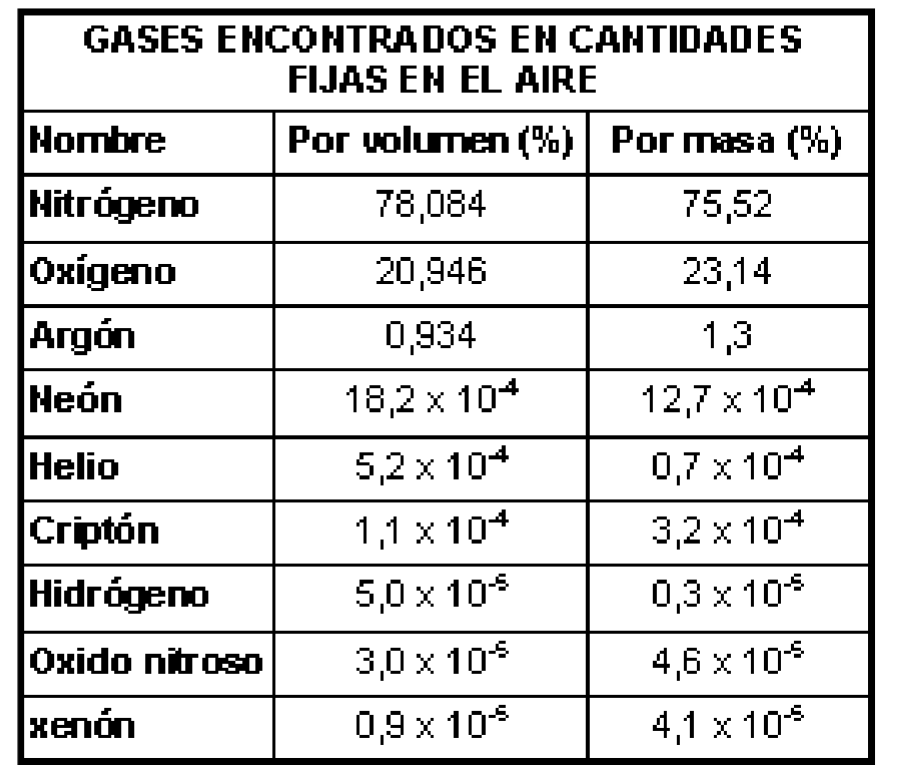
\includegraphics[width=0.5\textwidth]{imagenes/atm.png}
    \label{fig:composicion_atmosfera}
    \\
    \textbf{Contenido de vapor de agua varía entre 1-5\%}
\end{figure}

\subsection{Gases de efecto invernadero (GEI)}

\begin{itemize}
    \item Vapor de agua
    \item Dioxido de Carbono $CO_2$
    \item Metano $CH_4$
    \item Oxido Nitroso $N_2O$
    \item Ozono $O_3$
\end{itemize}

\subsection{Capas de la atmósfera}

\begin{enumerate}
    \item Troposfera: 0-13 km, contiene mayor parte del vapor de agua y es donde se desarrollan los fenómenos meteorológicos. Temperatura desciende hasta los -60°C.
    \item Estratosfera: 13-25 km, contiene la capa de ozono y temperatura constante a -60°C.
    \item Mesosfera: 25-80 km.
    \item Ionósfera: Absorbe las radiaciones de onda corta e ioniza moléculas.
    \item Exosfera: 500-1000 km, donde se encuentran los satélites. Se desvance gradualmente.
\end{enumerate}

\subsection{Circulación atmosférica}

Movimiento a gran escala de las masas de aire en la atm ocasionado por procesos térmicos y la rotación de la tierra.
\\\\
La energía que transmite el Sol a la Tierra no es homogénea. En los polos se reciben aprox. 90 $W/m^2$, mientras que en el ecuador se reciben 270 $W/m^2$. Esta diferencia provoca la transferencia de calor desde el ecuador a los polos, mediante celdas de convección y advección. Dado los continentes, mares y rotación, la transferencia de calor se realiza en 3 celdas:
\begin{itemize}
    \item Tropical
    \item Central
    \item Polar
\end{itemize}

\subsubsection{Celda de circulación vertical (Celda de Hadley)}

Como consecuencia de la diferencia de la distribución de energía en la tierra (radiación), el aire en el ecuador se calienta mucho más que el de los polos. 
\\\\
Si se supone tierra homogénea y en reposo, en el ecuador el aire al calentarse se eleva, a capas más altas, siendo sustituido por aire frio procedentes de los polos, ocurriendo una doble circulación de aire.

\begin{itemize}
    \item Del ecuador hacia los polos en las capas altas
    \item De los polos hacia el ecuador en las capas bajas
\end{itemize}

Esto no ocurre porque las masas de aire caliente al elevarse sufren un enfriamiento radiativo, provocando un aumento en su densidad y obligandolas a descender y calentarse adiabáticamente, conllevando una divergencia de dos subcorrientes superficiales, hacia el ecuador y hacia los polos.
\\\\
Esto define una celda cerrada en los trópicos (Celda de Hadley), con vientos del este hacia el ecuador (alisios) y vientos del oeste en altura a los polos (contraalisios).
\\\\
El aire que se mueve hacia los polos en el hemisferio sur adquiere un movimiento hacia el oeste, lo que ayuda a mantener la rotación de la Tierra. Cuando este aire llega a latitudes de 55°-60°, se encuentra con aire frío y seco que viene de los polos, formando el frente polar.
\\\\
El aire que converge hacia el frente polar asciende, creando dos nuevas celdas: una con corrientes hacia los polos (celda Polar) y otra con corrientes hacia el ecuador (celda Central).
\\\\
En realidad, la circulación general de la atmósfera se altera por la distribución de océanos y continentes, variaciones del relieve, vientos locales y sistemas de presión asociados a ciclones o anticiclones. Esto define los climas: secos en los polos y latitudes de 30º, y lluviosos en los trópicos.
\\\\
En Chile:

\begin{itemize}
    \item Zona Norte: Permanentemente bajo altas presiones. Desértica y bajas pps. 
    \item Zona Central: Mixto, húmeda en invierno y seca en verano
    \item Zona sur: Determianda por el frente polar. LLuvia siempre
    \item Zona polar: Alta presión, fría y seca. 
\end{itemize}

Las corrientes de mar dependen de los continentes y definen patrones de temperatura. Tienen efecto en el clima de una región.
En Chile, la corrinte de Humbolt es fría de S-N, modera las temperaturas.

\subsection{Presión atmosférica}

La presión atmosférica es el peso del aire sobre la superficie. Las curvas que representan igual presión se llaman isobaras, y su uso en cartas isobáricas permite caracterizar y predecir el clima.

\[
1 \, \text{atm} = 1 \, \text{bar} = 1.033 \, \text{kg/cm}^2 = 1013 \, \text{hPa} = 760 \, \text{mm Hg} = 14.7 \, \text{lb/in}^2
\]

\begin{equation}
    log(P_{atm}) = 2,882 - H/19500
\end{equation}

Donde $P_{atm}$ es la presión atmosférica (mm Hg) y H es la altitud (msnm)

\subsubsection{Centro de alta presión (Anticiclones)}

Proporcionan estabilidad atmosférica y constituyen barreras meteorológicas de desplazamiento de frentes, perturbaciones y tormentas.

\subsubsection{Centro de baja presión (Ciclones)}

Dan inestabilidades y perturbaciones atmosféricas que condicionan y suelen dar origen a precipitaciones y tormentas.

\section{Vientos}

Producen transferencias de calor y vapor de agua que condicionan fenómenos del ciclo hidrológico (Evaporación, evapotranspiración, derretimiento de nieves y hielos, formación de precipitaciones y desplazamiento de tormentas).
\\\\
Se originan por gradientes barométricos, en el sentido decreciente de dicho gradiente.
\\\\
Tipos de vientos:
\begin{itemize}
    \item Globales
    \item Regionales o locales
\end{itemize}

Los vientos de miden con un Anenómetro y la dirección se clasifica según su proveniencia
\\\\
Distribución del viento: dentro de la capa límite atmosférica

\begin{equation}
    \frac{v_1}{v_2} = \left(\frac{z_1}{z_2}\right)^p \quad \text{,} \quad p \approx \left[\frac{1}{7}, \frac{1}{3}\right]
\end{equation}

Si la atmósfera es neutra: Ley de von Kármán-Prandtl

\section{Radiación Solar}

\begin{itemize}
    \item Principal fuente energética para el desarrollo de los procesos físicos en la Tierra.
    \item La distribución estacional de esta energía depende de las características orbitales de la Tierra alrededor del Sol.
    \item Se propaga a la velocidad de la luz.
\end{itemize}

\subsection{Ley de Stefan Boltzmann}

La emisión total de radiación viene dada por la ecuación: 

\begin{equation}
    Re = e \times \sigma \times T^4
\end{equation}

Donde:
\begin{itemize}
    \item $e = $ emisividad de la superficie. ($e = 1$, cuerpo negro y $e = 0.97$, superficie del agua)
    \item $\sigma = 5.68 \times 10^{-8} (W/m^2 * K^4)$
    \item T = temperatura superficie en K  
\end{itemize}

\subsection{Ley de Wien}
La longitud de onda es inversamente proporcional a la temperatura de la superficie.

\begin{equation}
    \lambda (m) = 2.90 \times 10^{-3} / T (K)
\end{equation}

\subsection{Radiación neta}

La intensidad de la radicación solar que llega a la parte superior de la atmosfera disminuye por los siguientes factores: dispersión en la atmosfera, absorción en las nubes y oblicuidad de la sup. de la tierra

Se mide con:
\begin{itemize}
    \item Piranómetro: mide radiación solar global
    \item Piroheliómetro: mide radiación solar directa
    \item Piroradiómetro: mide radiación total incidente 
    \item Radiómetro neto: mide balance de radiación 
\end{itemize}

\section{Temperatura del Aire}

La temperatura es una medida de la energía interna de un cuerpo asociada al movimiento de partículas.
\\\\
La distribución de temperatura en la superficie y en la atm es resultado del balance energético global.
\\\\
Disminuye con la latitud y la altitud.
\\\\
En zonas marinas hay poca variación de la temperatura, en zonas áridas la variación es muy grande

\begin{align}
    \text{Si } Rad_{solar} > Emision_{Tierra} &\Rightarrow T \text{ aumenta} \\
    \text{Si } Rad_{solar} < Emision_{Tierra} &\Rightarrow T \text{ disminuye}
\end{align}

La temperatura del aire se mide por convección:
\begin{itemize}
    \item A 1,5 m de altura
    \item A la sombra y con ventilación
    \item En caseras meteorológicas
    \item Se mide con termómetro de mercurio
\end{itemize}

\subsection{Estimación de la temperatura}

\begin{itemize}
    \item Temperatura media diaria:
    \begin{equation}
        \bar{T} = \frac{T_{max} + T_{min} + T_{08} + T_{16}}{4}
    \end{equation}
    \item En ausencia de datos intermedios:
    \begin{equation}
        \bar{T} = \frac{T_{max} + T_{min}}{2}
    \end{equation}
    \item En alturas grandes se usan globosondas
    \item Gradiente adiabático normal: Tropósfera
    \begin{equation}
        \frac{\partial T}{\partial z} \approx -6{,}5 \, \left[\text{C/km}\right]
    \end{equation}
\end{itemize}

La única capa de interés es la tropósfera. Bajo ciertas condiciones se puede producir una inversión térmica, es decir que aumenta la T° con la altura.
\begin{itemize}
    \item Efecto del ciclo diurno
    \item Presencia de campos de hielon o nieve
    \item Poco viento
    \item Aire seco
    \item Pocas nubes
\end{itemize}

\section{Masas de aire y frentes}

Una masa de aire es un volumen de aire con propiedades físicas y termodinámicas uniformes horizontalmente. Estas masas adquieren características como temperatura y humedad en sus regiones de origen, y se modifican al mezclarse con otras masas de aire. La superficie frontal es la zona de separación entre masas de aire con diferentes propiedades. En Chile, las masas de aire provienen principalmente del océano Pacífico y regiones subpolares.
\\\\
Los frentes cálidos se forman cuando una masa de aire caliente se desplaza y asciende sobre una masa de aire más frío, generando precipitaciones extensas, que pueden abarcar entre 100 y 300 km en la zona del aire frío.
\\\\
Los frentes fríos ocurren cuando una masa de aire frío avanza sobre una masa de aire más cálido, provocando el ascenso del aire caliente. Las precipitaciones resultantes son generalmente intensas y cubren áreas pequeñas, de 60 a 80 km, en la zona previamente ocupada por el aire caliente.
\\\\
Frente Ocluido: cuando un frente frío alcanza a un frente cálido, el aire frío se desplaza por debajo del aire cálido, formando un frente ocluido. Las precipitaciones son intensas y cubren áreas pequeñas.

\subsection{Estabilidad Atmosférica}

\begin{itemize}
    \item Gradiente termico normal: $\gamma = -6,5 \, \text{(°C/km)}$
    \item Gradiente adiabático seco: $\Gamma_d = 9,8 \, \text{(°C/km)}$ Gas ideal y seco
    \item Graduente pseudo adiabático y humedo: $\Gamma_s$
    \begin{figure}[H]
        \centering
        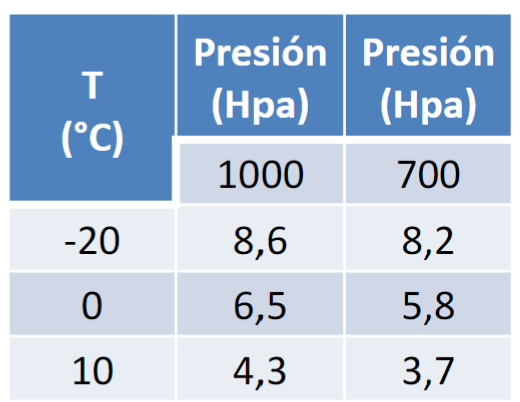
\includegraphics[width=0.3\textwidth]{imagenes/grad.png}
        \label{fig:gradiente}
    \end{figure}
\end{itemize}

La diferencia entre los gradientes tiene grandes implicancias en la estabilidad.
\\\\
Para que una masa de aire sea absolutamente estable, su gradiente de temperatura debe ser menor que el gradiente adiabático correspondiente: seco para aire seco y húmedo para aire saturado.

\begin{figure}[H]
    \centering
    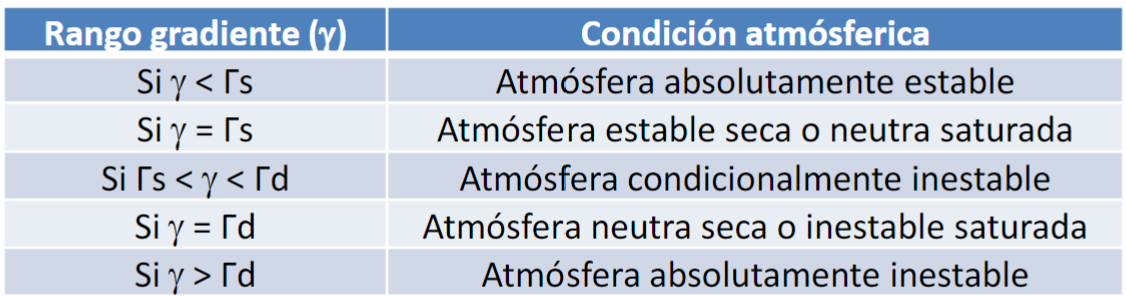
\includegraphics[width=0.5\textwidth]{imagenes/estabilidad.png}
    \label{fig:estabilidad}
\end{figure}

\section{Propiedades del vapor de agua}

Según la Ley de Dalton, la presión de vapor es la ejercida solo por el vapor de agua. La presión total de la atmósfera es la suma de la presión del aire seco y la del vapor de agua.

\begin{equation}
    e = \rho_v \cdot R_v \cdot T
\end{equation}

Donde:
\begin{itemize}
    \item $e = $ presión de vapor de agua (Pa)
    \item $\rho_v = $ densidad del vapor de agua (gr/m³)
    \item $R_v = $ constante de los gases para vapor de agua (J/kg K)
    \item $T = $ temperatura (K)
\end{itemize}

\begin{equation}
    P_{total} = P_{seco} + e
\end{equation}

\begin{equation}
    P_{seco} = \rho_d \cdot R_d \cdot T
\end{equation}

Donde: 
\begin{itemize}
    \item $\rho_d$ es la densidad del aire seco (gr/m³)
    \item $R_d$ es la constante de los gases para aire seco = 287 (J/kg K)
\end{itemize}

\begin{equation}
    P_{total} = \rho_d \cdot R_d \cdot T + \rho_v \cdot R_v \cdot T \quad ; \quad R_v = \frac{R_d}{0.622}
\end{equation}
    
\begin{equation}
    P_{total} = \rho_d \cdot R_d \cdot T + \rho_v \cdot \left(\frac{R_d}{0.622}\right) \cdot T
\end{equation}
    
\begin{equation}
    P_{total} = \left(\rho_d + \frac{\rho_v}{0.622}\right) \cdot R_d \cdot T
\end{equation}

Humedad específica: 
\begin{equation}
    q_v = 0,622 \cdot \frac{e}{P}
\end{equation}

\begin{equation}
    R_a = R_d \cdot \left(1 + 0.608 \cdot q_v \right)
\end{equation}

Para una temperatura del aire dada, el contenido máximo de humedad que el aire puede contener corresponde a la presión de vapor de saturación (\(e_s\)), que se puede calcular con una ecuación específica.

\begin{equation}
    e_s = 611 \cdot \exp\left(\frac{17.27 \cdot T}{237.3 + T}\right)
\end{equation}

Humedad relativa:
\begin{equation}
    R_h = \frac{e}{e_s}
\end{equation}

Temperatura de punto de rocío (\(T_d\)): es la temperatura a la que se debe enfriar una masa de aire húmedo para que se sature, manteniendo la misma presión y contenido de agua.
\\\\
Punto de rocío: temperatura a la que habría que enfriar el aire, manteniendo constante la presión de vapor, para que se sature. En este punto se cumple:

\begin{equation}
    e = e_s \cdot T_R
\end{equation}

\section{Humedad Atmosférica}










\part{Capitulo 4}
\vspace{-0.3cm}
\begin{center}
    \begin{large}
        Metodos Probabilisticos y Estadisticos
    \end{large}
\end{center}

La mayor parte de los procesos hidrologicos son aleatorios, no existen procesos puramente deterministicos. En consecuencia, para poder hacer una caracterizacion se \textbf{debe registrar la ocurrencia de ellos} mediante registros historicos, los cuales son sometidos a un post procesado estadistico.
\\ \\
Los objetivos son los siguientes:

\begin{itemize}
    \item Estimacion de P( ) de que ocurra un determinado evento
    \item Estimacion de eventos que no han ocurrido o no se han observado
    \item Caracterizacion estadistica de series hidrologicas
    \item Correlacion y regrecion para completar y extender series
\end{itemize}

\section{Frecuencia Relativa y Acumulada}

La sumatoria de todas las frecuencias relativas debe ser igual a 1, es decir:

\begin{equation}
    \sum_{i=1}^{n} f_i = 1
\end{equation}

Estas funciones son obtenidas a partir de una muestra, por lo que se pueden obtener de estimaciones de la poblacion aproximando como limites:

\begin{figure}[H]
    \centering
    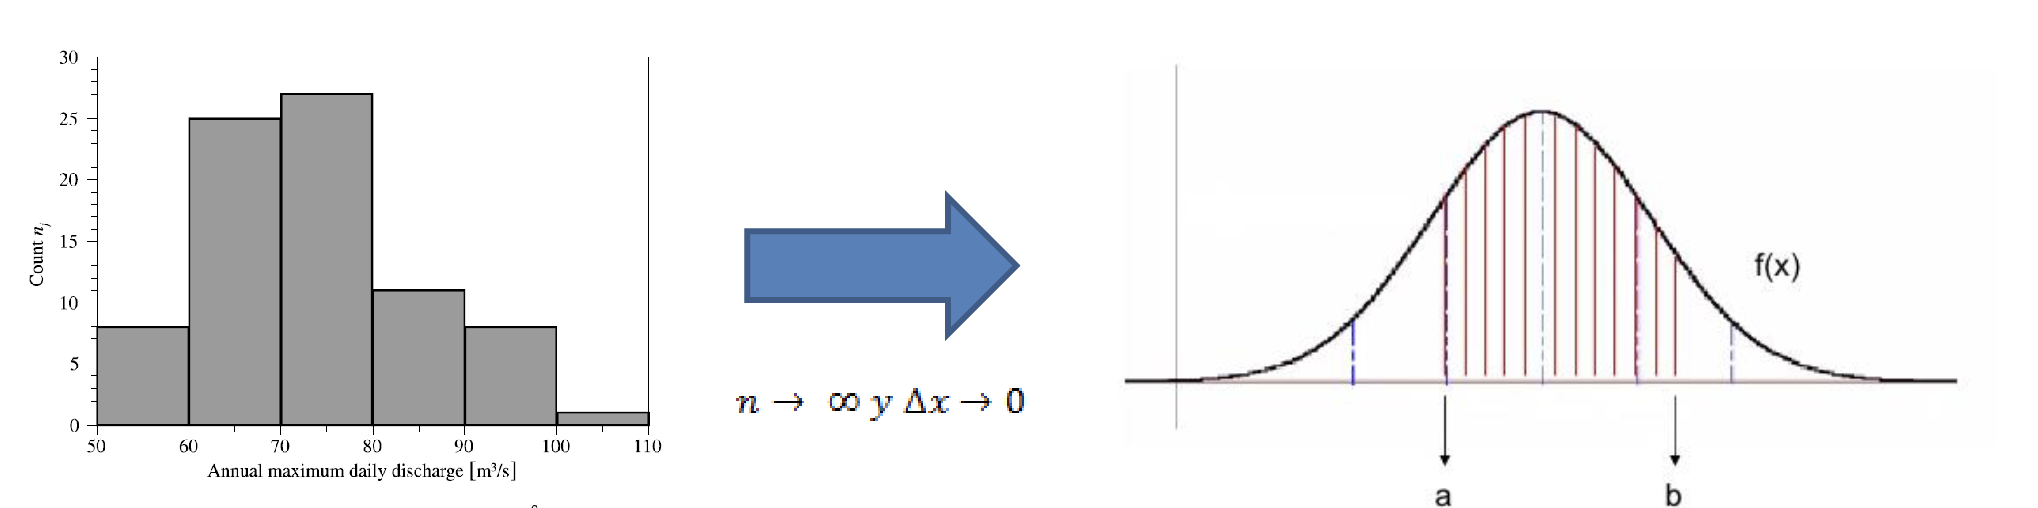
\includegraphics[width=0.85\textwidth]{imagenes/frecuencia.png}
    \label{fig:frecuencia_acumulada}
\end{figure}

\section{Periodo de Retorno y P( ) de Excedencia}

Se puede definir como: el intervalo de recurrencia promedio entre evnetos que igualan o excedan una magnitud especifica
\\ \\
Es decir, en un horizonte de tiempo grande, se esperaria observar eventos iguales o mayores cada \textbf{T años}.
\\ \\
Sea \textbf{p} la probabilidad de exito y \textbf{(1-p)} la probabilidad de falla en un determinado año. Podemos definir la \textbf{probabilidad de recurrencia $\pi$} como el producto de \textbf{$\pi$ - 1} fallas seguidas por un exito, por lo tanto:

\begin{equation}
    P(X > X_t) = \frac{1}{T}
\end{equation}

Ejemplo:

\begin{figure}[H]
    \centering
    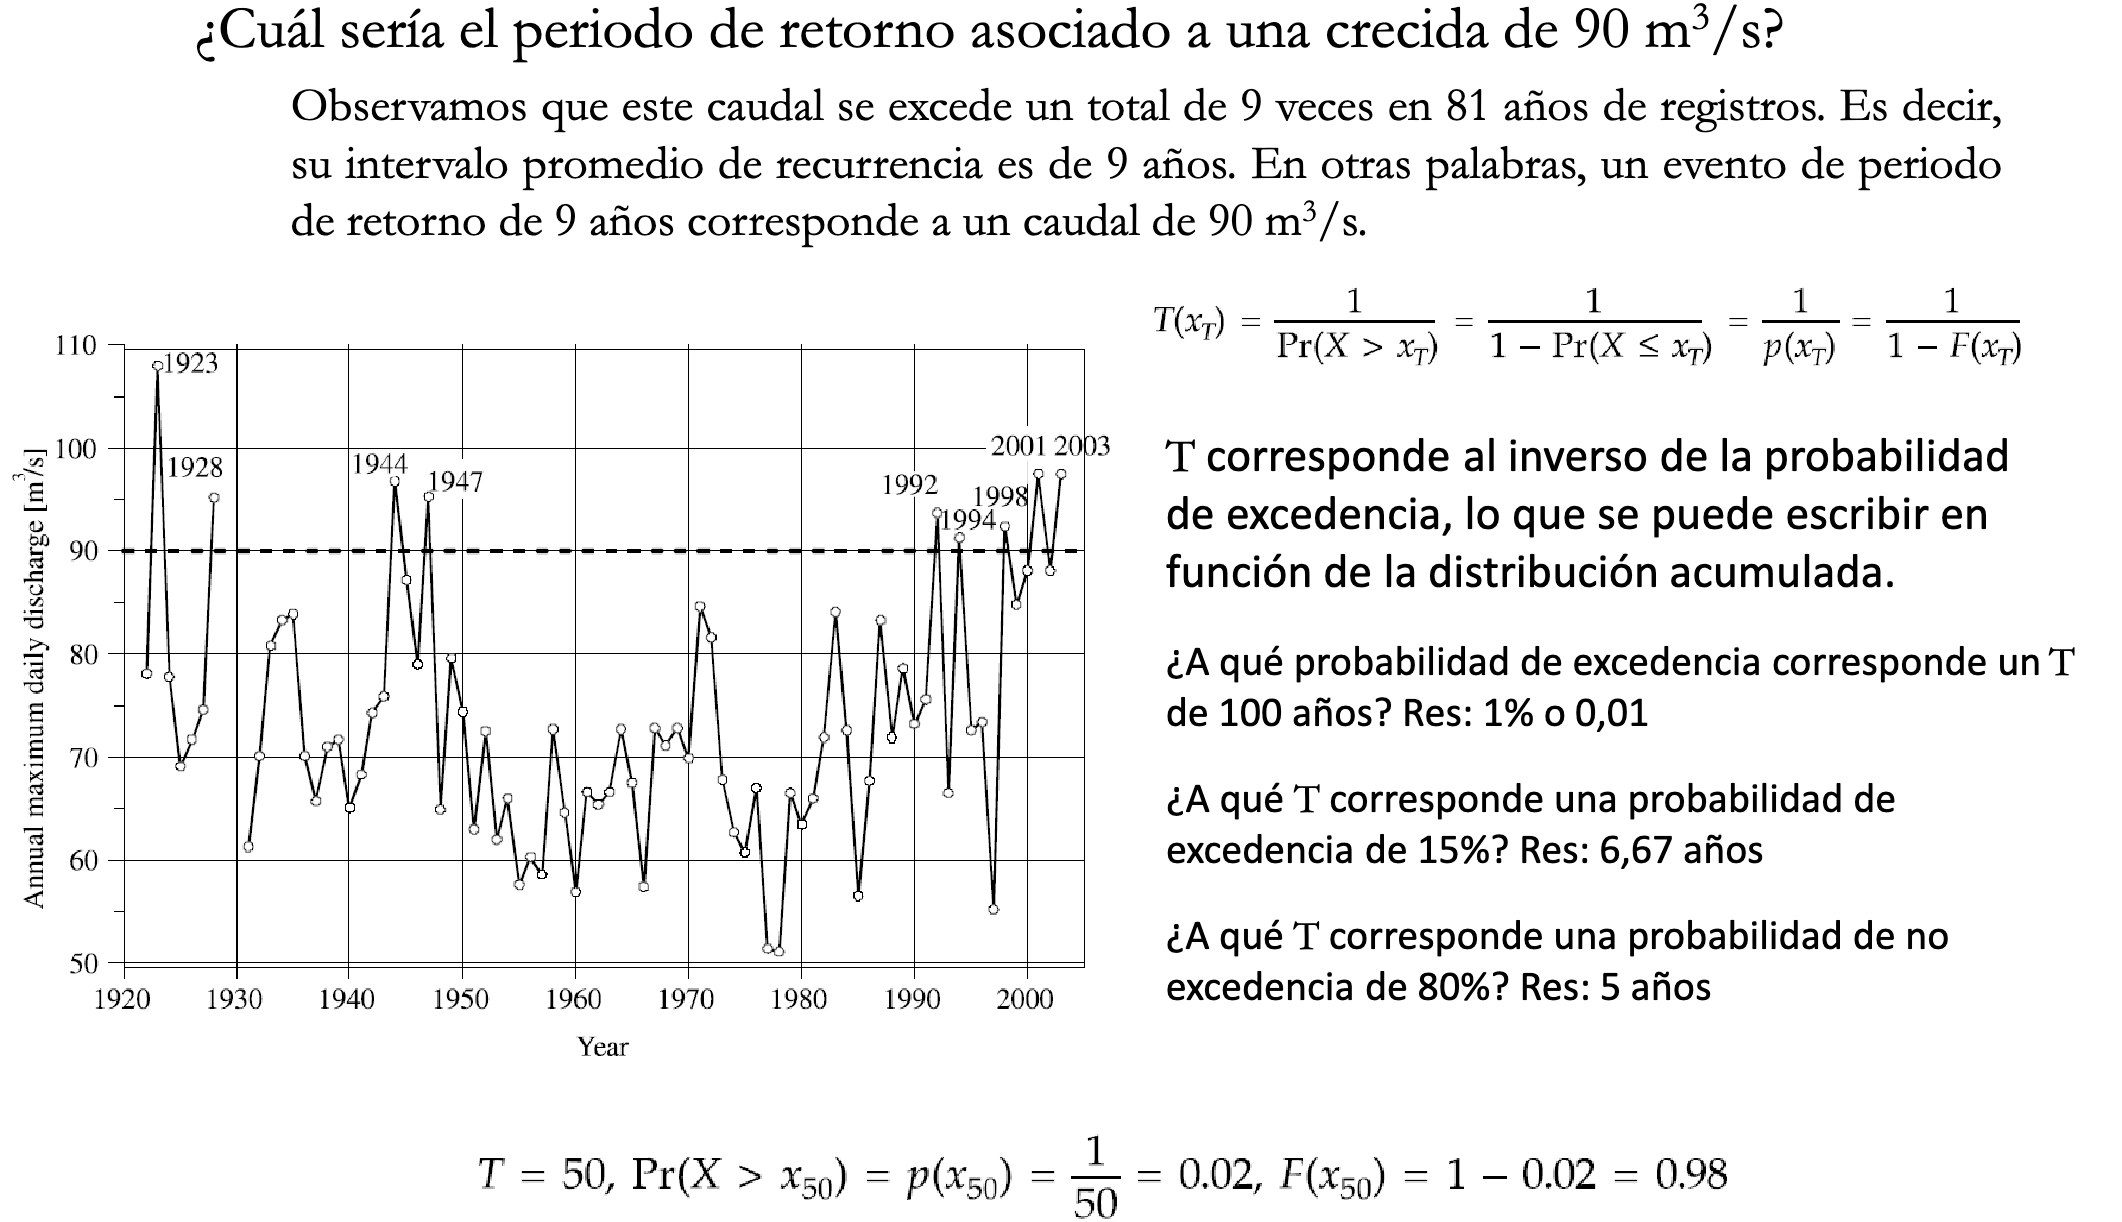
\includegraphics[width=0.85\textwidth]{imagenes/retorno.png}
    \label{fig:periodo_retorno}
\end{figure}

\section{Seguridad y Riesgo Hidrololgico}

Se define como la probabilidad de no excedencia:

\begin{equation}
    P_{no-exc} = 1 - \frac{1}{T}
\end{equation}

Por lo tanto, la probabilidad de que cierto valor no se exceda en n años es:

\begin{equation}
    S = (1 - \frac{1}{T})^n 
\end{equation}

Lo cual se define como \textbf{Seguridad Hidrologica}, donde su complemento es el \textbf{Riesgo Hidrologico}, lo cual se usa para obras hidraulicas:

\begin{equation}
    R = 1- S = 1 - (1 - \frac{1}{T})^n
\end{equation}

\textbf{Nota: aproximar el valor de t a un valor multiplo de 5}

\section{Distribuciones Discretas}

\subsection{Bernoulli}

Una variable aleatoria posee dos estados, exito o fracaso, por lo tanto puede ser 1 o 0. Por lo tanto:

\begin{equation}
    P(X = 1) = p
\end{equation}

\begin{equation}
    P(X = 0) = 1 - p
\end{equation}

\subsection{Distribucion Binomial}

Este modelo surge a partir de la realizacion de n ensayos independientes tipo bernoulli, donde se define una variable aleatorioa k como el numero de exitos que ocurren en n ensayos, por lo tanto:

\begin{equation}
    P(X = k) = \binom{n}{k} \cdot p^k \cdot (1-p)^{n-k}
\end{equation}

Donde:

\begin{equation}
    \binom{n}{k} = \frac{n!}{k!(n-k)!}
\end{equation}

Y K es el numero de evnetos exitosos.
\\ \\
Cada evento climatologico es independiente, por lo tanto es un ensayo tipo bernoulli, y su conjunto se representa binomialmente

\section{Parametros Estadisticos}

\subsection{Varianza}

Se denomina a la varianza \textbf{$s^2$} como la media de los cuadrados de las diferencias entre cada valor y la media, por lo tanto:
\\ \\
Caso discreto: 

\begin{equation}
    s^2 = \frac{\sum_{i=1}^{n} (x_i - \bar{x})^2}{n-1}
\end{equation}

Caso continuo:

\begin{equation}
    \sigma^2 = E((x-\mu)^2)
\end{equation}

\subsection{Desviacion Estandar}

Se define como la raiz cuadrada de la varianza, por lo tanto:

\begin{equation}
    s = \sqrt{s^2}
\end{equation}

\subsection{Coeficiente de Variacion}

Se define como la relacion entre la desviacion estandar y la media, por lo tanto:

\begin{equation}
    CV = \frac{s}{\bar{x}}
\end{equation}

\subsection{Coeficiente de Asimetria}

Se define como la medida de asimetria de una distribucion, por lo tanto:

\begin{equation}
    \gamma = \frac{E((x-\mu)^3)}{\sigma^3}
\end{equation}

\section{Distribuciones Continuas}

\subsection{Distribucion Normal}

Se define como:

\begin{equation}
    f(x) = \frac{1}{\sigma\sqrt{2\pi}} \cdot e^{-\frac{(x-\mu)^2}{2\sigma^2}}
\end{equation}

Donde $\mu$ es la media y $\sigma$ la desviacion estandar.
\\ \\
Esta funcion no es integrable, por lo tanto para evaluar la funcion se utilizan tablas y o formulas aproximadas.
\\ \\
\textbf{El proceso de normalizacion consiste en reemplazar la variable original por una nueva variable estandarizada (z) }

\begin{equation}
    z = \frac{x-\mu}{\sigma}
\end{equation}

De esta forma se obtiene:

\begin{equation}
    f(x) = \frac{1}{\sqrt{2\pi}} \cdot e^{-\frac{z^2}{2}}
\end{equation}

\subsection{Distribucion Log Normal}

Es una transformacion de la distribucion Normal, donde se modela de una forma asimetrica con respecto a un valor medio, por ejemplo para precipitaciones o caudales:

\begin{equation}
    f(x) = \frac{1}{\sigma_y\sqrt{2\pi}} \cdot e^{\frac{1}{2}(\frac{y-\mu_y}{\sigma_y})^2}
\end{equation}

Donde los parametros se estiman en base a la muestra aplicando log a las variables observadas:

\begin{equation}
    \mu_y = \bar{y} = \frac{1}{N} \sum_{i=1}^{N} \ln(x_i)
\end{equation}



\part{Capitulo 5}

\part{Ayudantia 1}

Se define el balance hidrologico general como:

\begin{equation}
    \frac{ds}{dt} = X_{Entrada}-Y_{Salida}
\end{equation}

Lo cual se puede desglozar en 4 terminos:

\begin{equation}
    \Delta S_L + \Delta S_S + \Delta S_Z + \Delta S_N = P + Q_{SA} + Q_{ZA} - (E +ET +Int + Q_{SE} + Q_{ZE})
\end{equation}

Donde:

\begin{itemize}
    \item $\Delta S_L$: Cambio de almacenamiento superficial como lagos o embalses
    \item $\Delta S_S$: Cambio de almacenamiento de suelo no subterraneo
    \item $\Delta S_Z$: Cambio de almacenamiento de suelo subterraneo
    \item $\Delta S_N$: Cambio de almacenamiento de nieve y glaciares
    \item P: Precipitacion
    \item $Q_{SA}$: Caudal Superficial Afluente
    \item $Q_{ZA}$: Caudal Subterraneo Afluente
    \item E: Evaporacion
    \item ET = Evapotranspiracion
    \item Int: Infiltracion
    \item $Q_{SE}$: Caudal Superficial Efluente y caudal subterraneo efluente
\end{itemize}

Donde se define como:

\begin{itemize}
    \item Efluente: Caudal que sale de un sistema
    \item Afluente: Caudal que entra a un sistema
\end{itemize}

Se define como \textbf{acumulacion}:

\begin{equation}
    \frac{dv}{dt} = \frac{A\Delta H}{dt}= Q_A + P - (Q_E + Q_{ZE} + E)
\end{equation}

Con eso se puede obtener el aumento o disminucion de altura de un embalse.

\part{Ayudantia 2}

\section{Parte 1}

Si tenemos un caso donde conocemos 2 puntos a alturas distinta:

\begin{figure}[H]
    \centering
    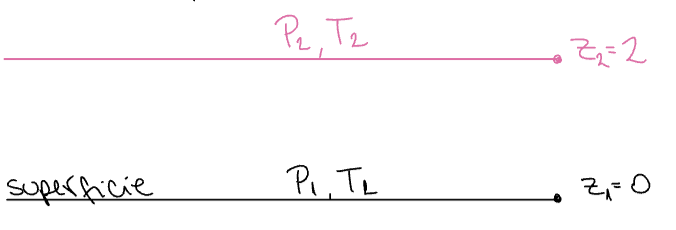
\includegraphics[width=0.5\textwidth]{imagenes/ayud_2_1.png}
    \label{fig:altura}
\end{figure}

Podemos determinar el agua precipitable se utiliza la siguiente formula:

\begin{equation}
    \Delta m_p = q_v \cdot p_a \cdot A \cdot \Delta Z
\end{equation}

$q_v$ se define como:

\begin{equation}
    q_v = 0.622 \cdot \frac{e}{p_a}
\end{equation}

Donde e es la presion de vapor y $p_a$ es la presion atmosferica.
\\ \\ 
Ademas, se tiene lo siguiente:

\begin{equation}
    HR = \frac{e}{e_s} \cdot 100
\end{equation}

Donde HR es la humedad relativa y $e_s$ es la presion de vapor de saturacion, de lo cual se obtiene:

\begin{equation}
    e_s = 611^(\frac{17.27 \cdot T}{237.3 + T})
\end{equation}

Los valores de e y $e_s$ son en pascales, donde las temperaturas son ingresadas en celcius.
\\ \\
Donde podemos calcular la presion del punto mas alto en variacion al punto base de referencia:

\begin{equation}
    P2 = P1 \cdot (\frac{T2}{T1})^(\frac{g}{\alpha \cdot Ra})
\end{equation}

Donde $\alpha$ ($\frac{C}{Km}$) es el gradiente de temperatura, Ra $\frac{J}{Kg \cdot K}$ es la constante de los gases y g es la gravedad.
\\ \\
Podemos conocer la temparatura en el punto de segun la temparatura en el punto 1:

\begin{equation}
    T2 = T1 + \alpha \cdot \Delta Z
\end{equation}

Ademas, es nesesario calcular la presion en el punto base de referencia segun la Ra y T:

\begin{equation}
    P1 = \frac{P1}{Ra \cdot T1}
\end{equation}

Lo mismo es nesesario hacer con P2.
\\ \\
Luego, como en este caso hay 2 puntos, hay que sacar el promedio de $q_v$ y Pa, obteniendo asi $\Delta m_p$.  

\section{Parte 2}

Podemos obtener la vida util a partil de la seguridad:

\begin{equation}
    S = (1 - \frac{1}{T})^n
\end{equation}

\subsection{Gumbell}

Se define Gumbell como:

\begin{equation}
    X_T = \mu + K_t \cdot \sigma
\end{equation}

\begin{equation}
    K_t = \frac{y_t - y_n}{\sigma_n}
\end{equation}

Usar los siguientes valores:

\begin{figure}[H]
    \centering
    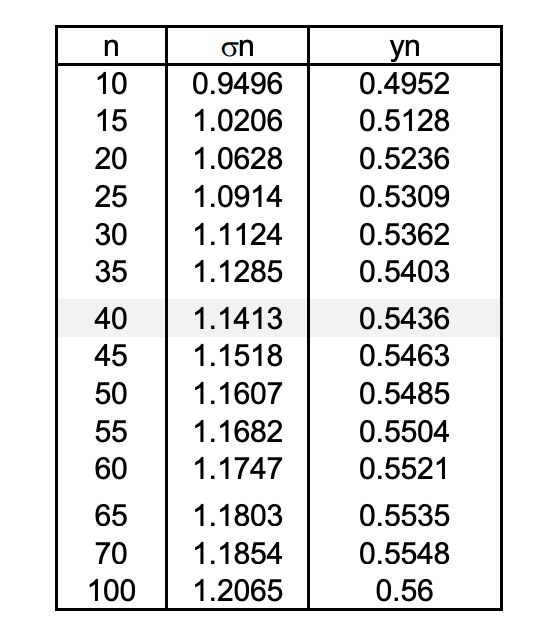
\includegraphics[width=0.5\textwidth]{imagenes/tabla_valores_gumbell.jpg}
    \label{fig:valores}
\end{figure}

\begin{equation}
    y_t = -\ln(\ln(\frac{T}{T-1}))
\end{equation}

Los valores n deben ser entregados.
\\ \\
La probabilidad de que la estructura falle mas de \textbf{X} veces es:

\begin{equation}
    P(X_{fallas}) = 1 - P(0) + P(1) + P(2) + ... + P(X-1)
\end{equation}

Aplicando la distribucion de bernoulli:

\begin{equation}
    P(k) = \binom{n}{k} \cdot P^k \cdot (1-P)^{n-k}
\end{equation}

Donde \textbf{k es el numero de fallas} y \textbf{P las probabilidades de excedencia}.

\begin{equation}
    \binom{n}{k} = \frac{n!}{k!(n-k)!}
\end{equation}

\subsection{Log Pearson III}

Se define como:

\begin{equation}
    X_T = \mu + K_t \cdot \sigma
\end{equation}

\begin{equation}
    K_t = Z + (Z^2 - 1)K + \frac{1}{3}(Z^3 - 6Z)K^2 - (Z^2-1)K^3 + Z\cdot K^4 + \frac{K^5}{3}
\end{equation}

\begin{equation}
    K = \frac{CS}{6}
\end{equation}

Donde CS es el coeficiente de simetria.
\\ \\
Z se calcula de acuerdo a la distribucion normal:

\begin{equation}
    Z = W -  \frac{2.516 + 0.803W + 0.0103W^2}{1 + 1.432W + 0.189W^2 + 0.001308W^3}
\end{equation}

\begin{equation}
    W = (\ln(\frac{1}{P^2}))^{0.5}
\end{equation}

\begin{equation}
    P = \frac{1}{T}
\end{equation}

\subsection{Caudal de Diseño}

Luego usando las distintas distribuciones, se define el caudal de diseño como:

\begin{equation}
    Q_{diseno} = \exp(X_T)
\end{equation}

\subsection{Intervalos de Confianza}

Se define como:

\begin{equation}
    X_t + - S_e \cdot Z_{\alpha}
\end{equation}

\textbf{$Z_{\alpha}$} es la variable normal estandar para un nivel de confianza de $\alpha$. Para $\alpha$ = 5 \%, implica que $Z_{\alpha}$ = 1.96. = 1.645. Luego:

\begin{equation}
    S_e = \sqrt{(1+1.139K_t + 1.1000K_t^2) \cdot \frac{1}{n}}
\end{equation}

De esta forma, obtenemos los 2 limites del intervalo de confianza.

\newpage
\bibliography{referencias}  % Nombre del archivo .bib

\end{document}
